\documentclass{article}
\usepackage{listings}
\usepackage{xcolor}
\usepackage{pagecolor}
\usepackage{hyperref}
\usepackage{graphicx}
\usepackage{titling}

\title{\Huge\bfseries Web-Crawler Documentation}
\author{Omkar Shirpure (22B0910)}
\date{}

\definecolor{codegreen}{rgb}{0,0.6,0}
\definecolor{codegray}{rgb}{0.5,0.5,0.5}
\definecolor{codepurple}{rgb}{0.58,0,0.82}
\definecolor{backcolour}{rgb}{0,0,0}
\definecolor{stringcolor}{rgb}{0.0,0.7,0.0}
\definecolor{commentcolor}{rgb}{0.5,0.5,0.5}
\definecolor{keywordcolor}{rgb}{0.0,0.7,0.0}
\definecolor{linkcolor}{rgb}{0.8,0.8,0.8}

\lstdefinestyle{mystyle}{
    backgroundcolor=\color{backcolour},
    commentstyle=\color{commentcolor},
    keywordstyle=\color{keywordcolor},
    numberstyle=\tiny\color{codegray},
    stringstyle=\color{stringcolor},
    basicstyle=\ttfamily\small,
    breakatwhitespace=false,
    breaklines=true,
    captionpos=b,
    keepspaces=true,
    numbers=left,
    numbersep=5pt,
    showspaces=false,
    showstringspaces=false,
    showtabs=false,
    tabsize=2
}

\pagecolor{backcolour}
\color{stringcolor}

\lstset{style=mystyle}

\begin{document}

\begin{titlingpage}
\maketitle
\vspace{2cm}
\centering
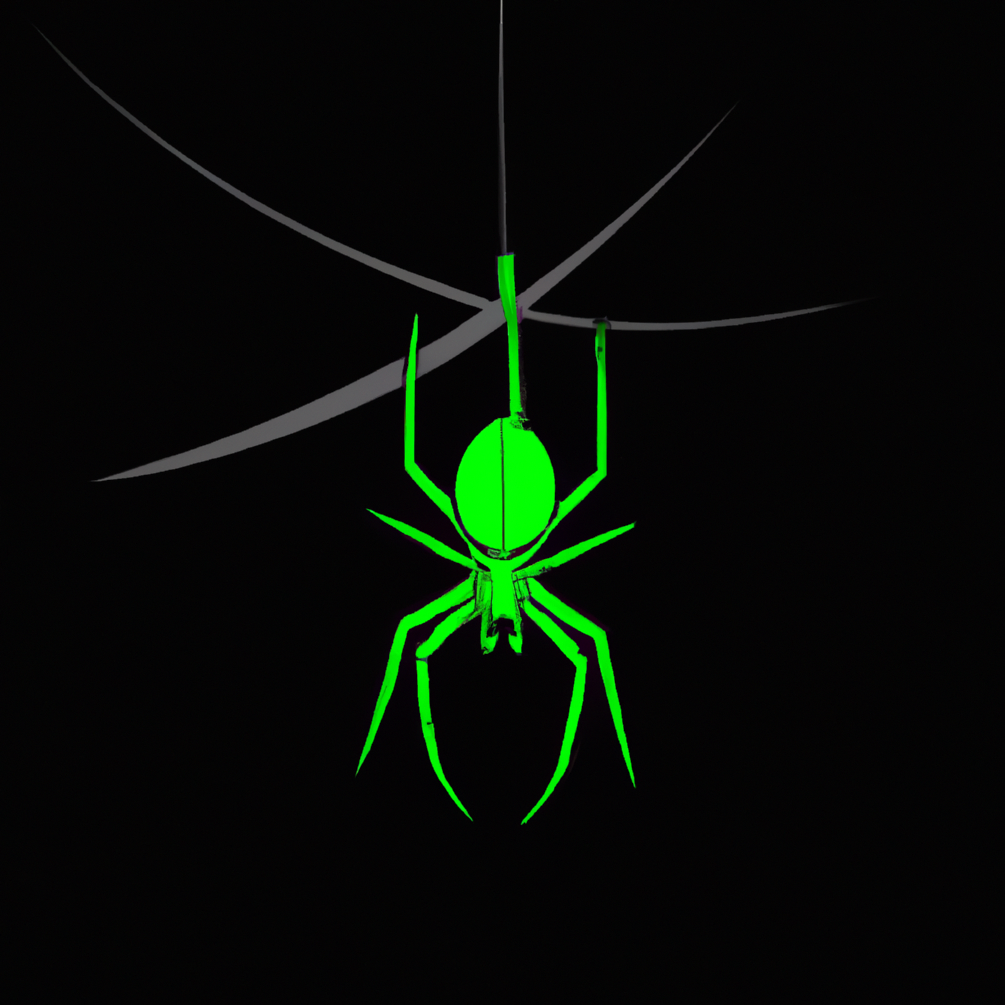
\includegraphics[width=0.6\linewidth]{spider.png}
\end{titlingpage}


\newpage

\tableofcontents

\newpage

\section{Introduction}
The Web-Crawler is a Python program designed as the culmination of a comprehensive course on web development and data extraction. This end-of-semester project aimed to assess the students' mastery of the skills learned throughout the course. The Web-Crawler tackles the problem of efficiently extracting information from websites, addressing the challenges of navigating through webpages, retrieving links, and collecting data on various file types. By automating these tasks, the Web-Crawler serves as a practical demonstration of the students' abilities to apply their acquired knowledge and skills to real-world scenarios.

\vspace{0.6in}
\section{How to Use the Web-Crawler}
To use the Web-Crawler program, follow these steps:

\begin{enumerate}
    \item Open a command-line interface.
    \item Run the Python script with the following command: \texttt{python web\_crawler.py}
    \vspace{\baselineskip}


    \texttt{without find function: }
    
    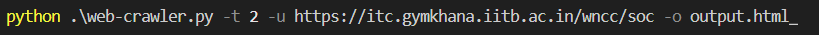
\includegraphics[width=0.9\linewidth]{sc1.png}

    
    \texttt{with find function: }

    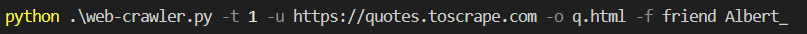
\includegraphics[width=0.9\linewidth]{sc2.png}
    \item Provide the required command-line arguments:
    \begin{itemize}
        \item \texttt{-u} or \texttt{--url}: The URL of the website to crawl.
        \item \texttt{-t} or \texttt{--threshold}: The recursion threshold (maximum depth) for crawling.
        \item \texttt{-o} or \texttt{--output}: (Optional) The output file name to save the HTML flow chart. If not provided, the flow chart will be displayed in the console.
        \item \texttt{-f} or \texttt{--find}: (Optional) One or more keywords to search for in the links. Only links containing these keywords will be displayed in the flow chart.
    \end{itemize}
    \item Press Enter to execute the program.
    \item The program will crawl the website and generate an HTML flow chart displaying the links and files found. If an output file name is provided, the flow chart will be saved to that file; otherwise, it will be displayed in the console.
\end{enumerate}

\section{Output}
\texttt{The output in the terminal}

\vspace{0.2cm}
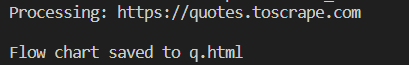
\includegraphics[scale=0.7]{sc3.png}

\vspace{1cm}
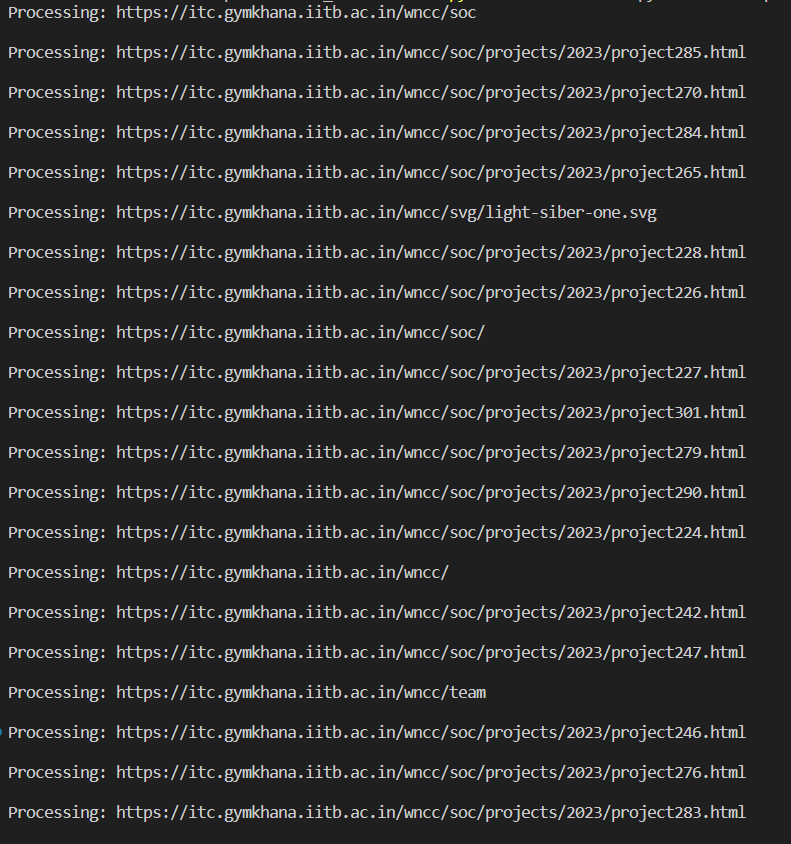
\includegraphics[scale=0.7]{qq (1).png}
\vspace{4cm}

\texttt{Output in the HTML to display the links and browse easily :}

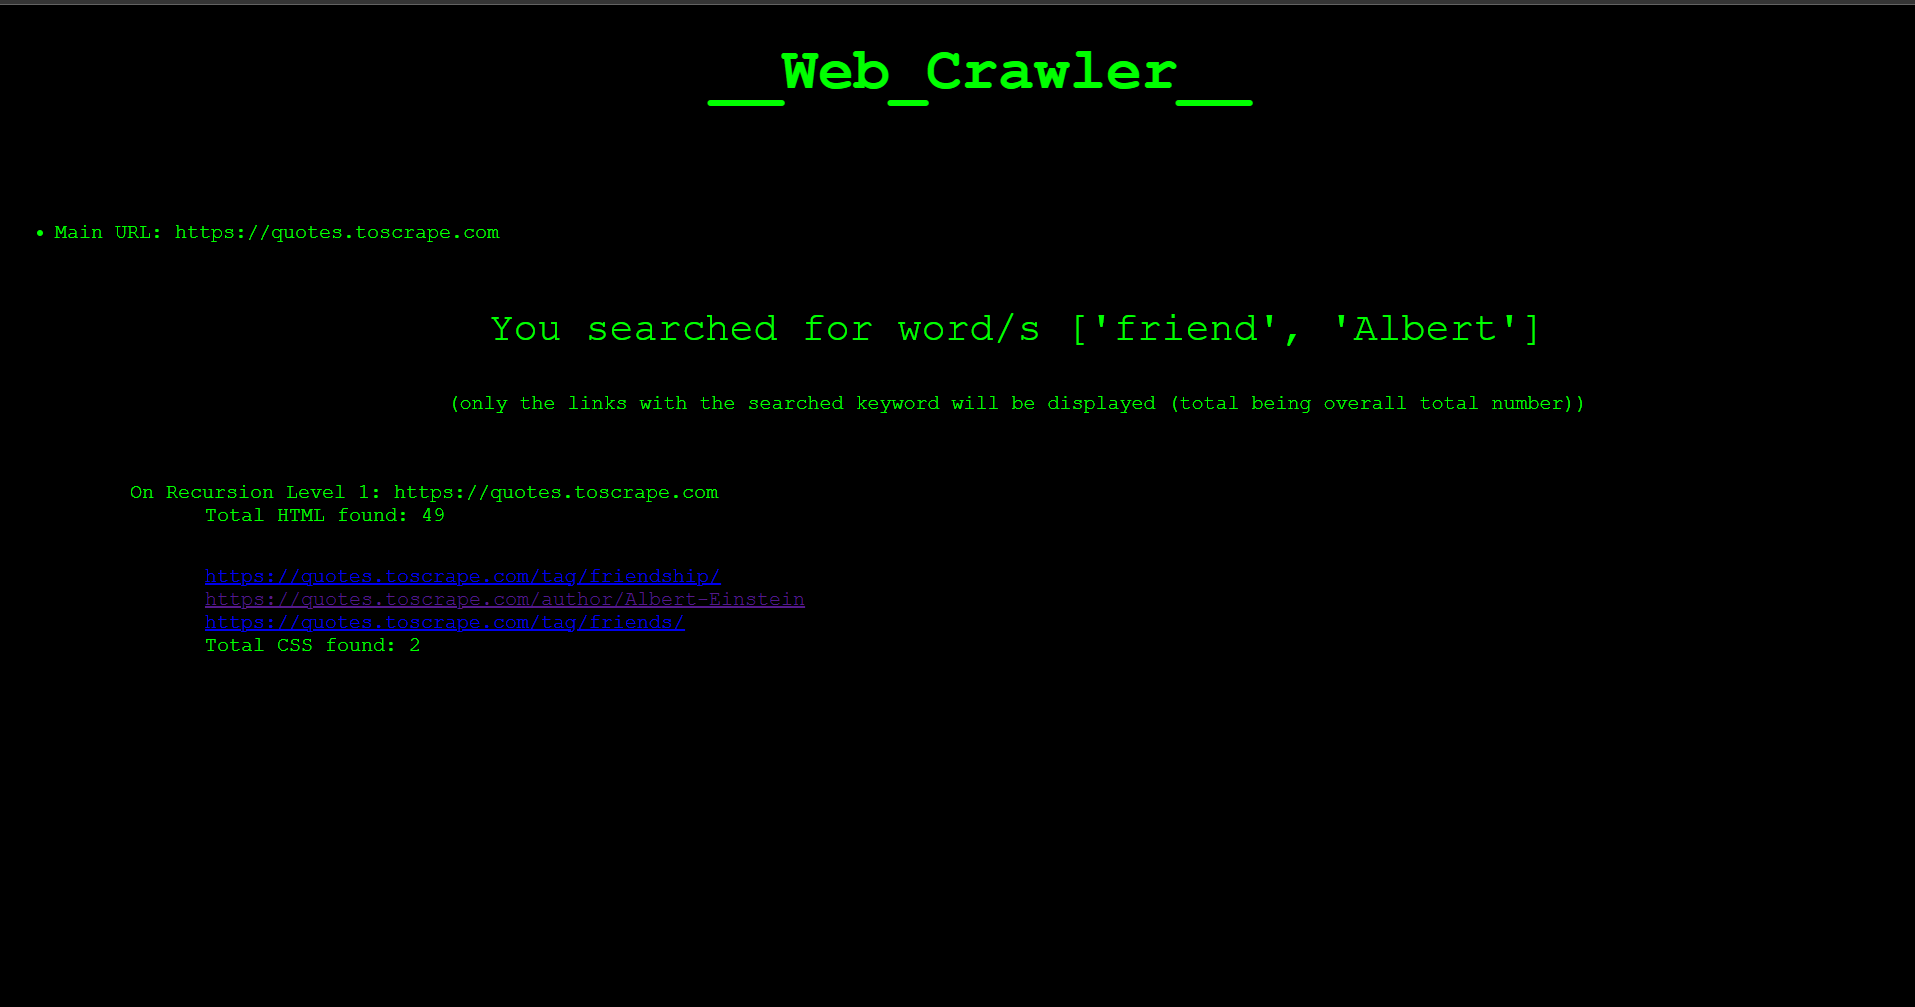
\includegraphics[scale=0.4]{qq (2).png}

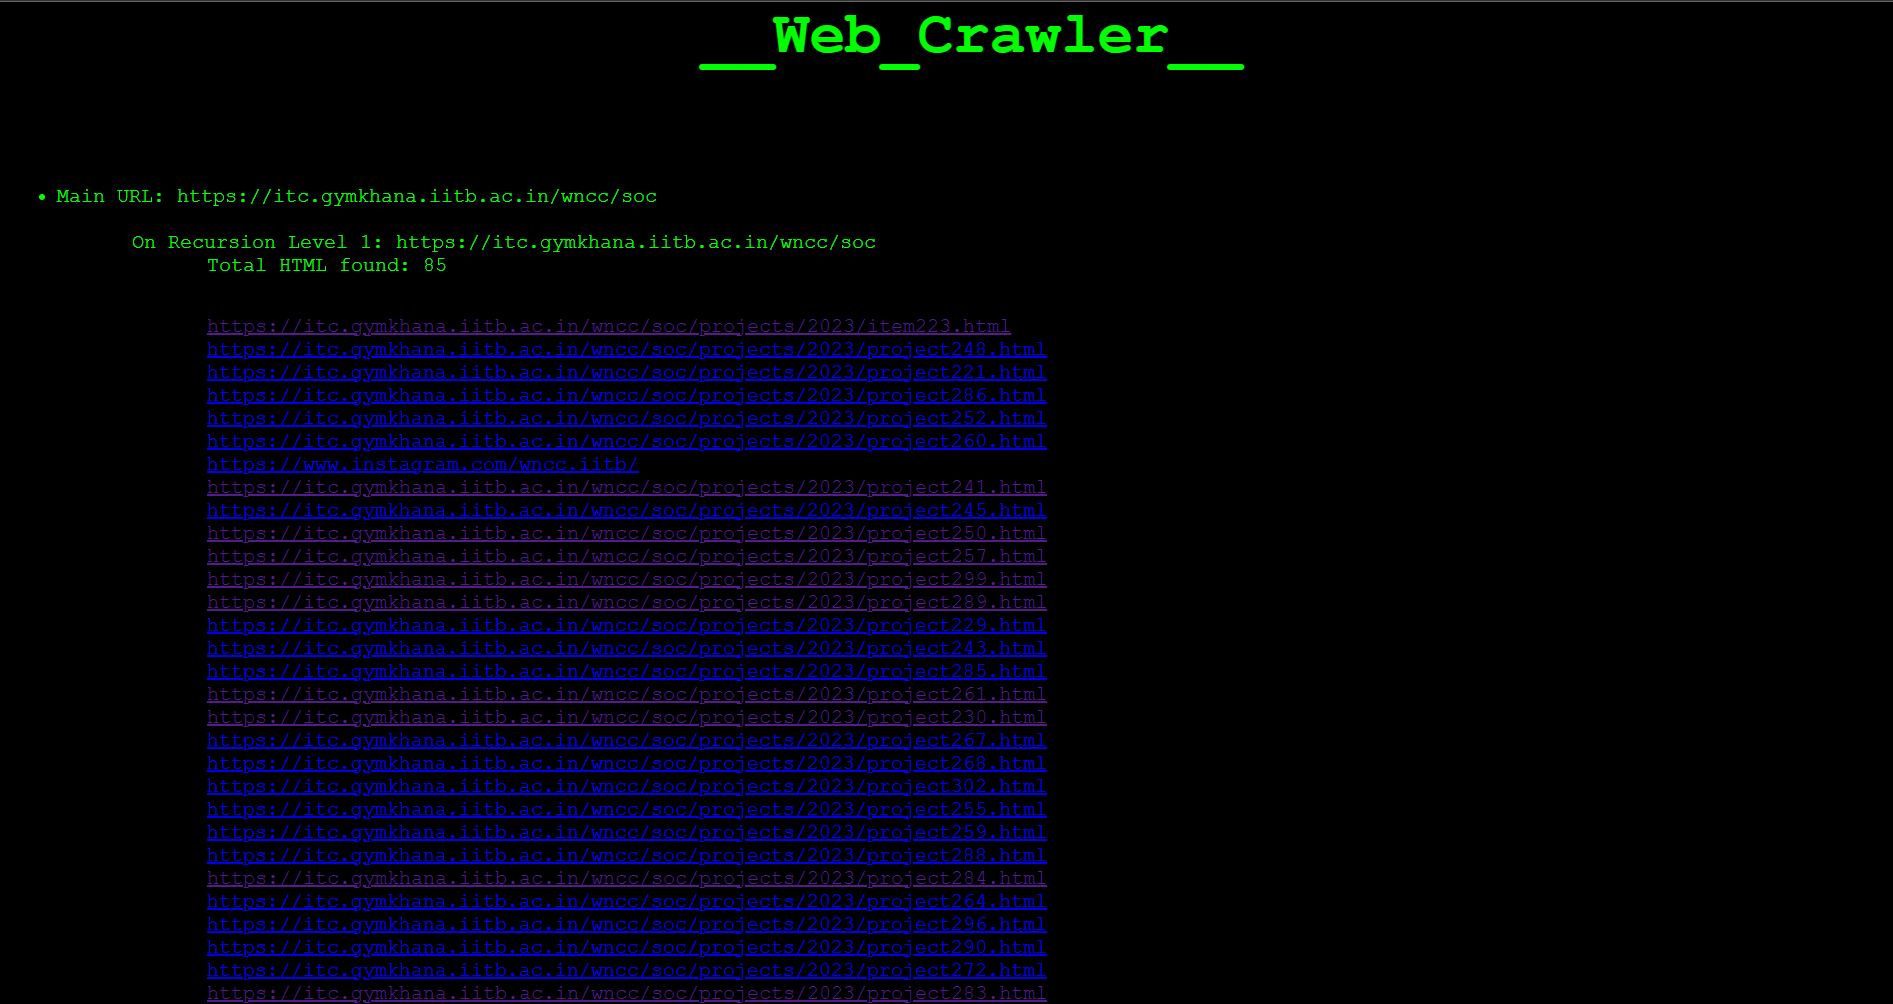
\includegraphics[scale=0.4]{qq (3).png}

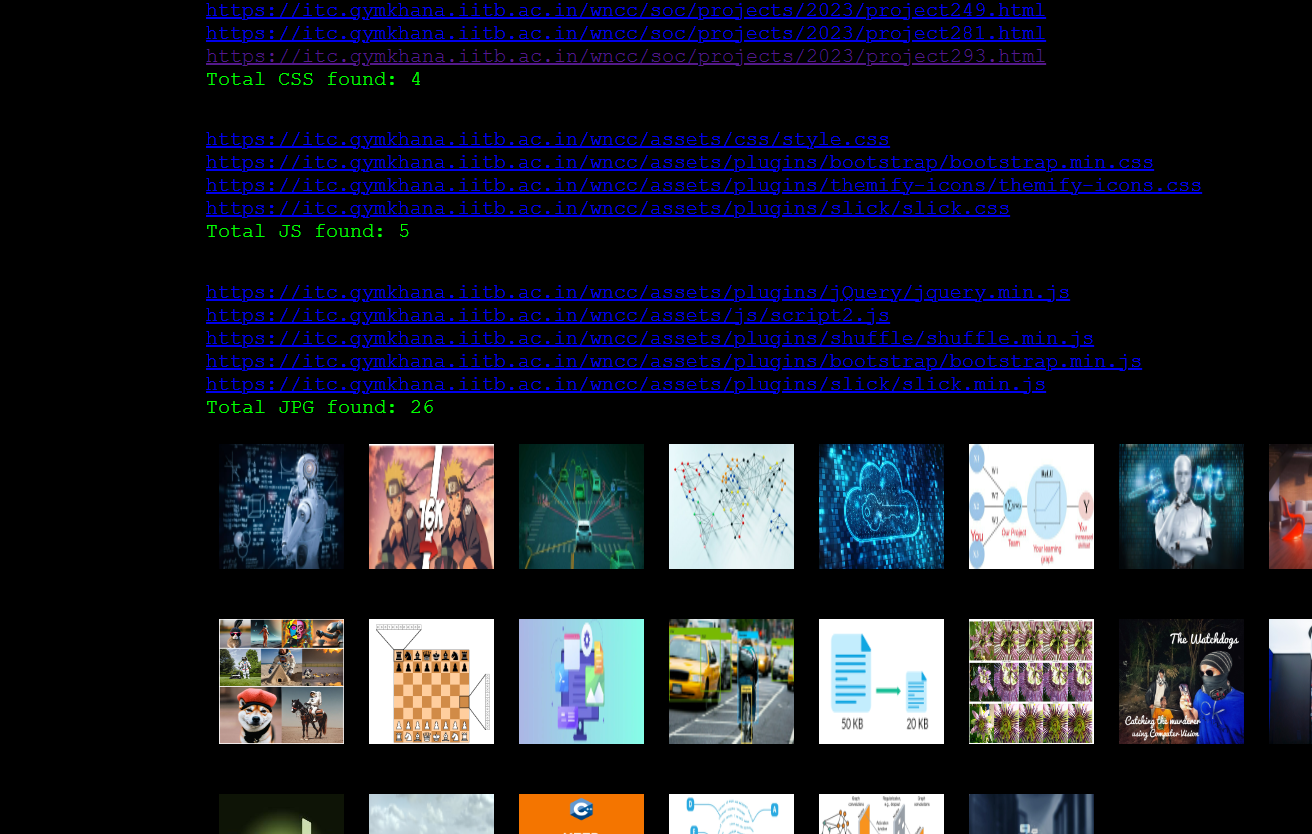
\includegraphics[scale=0.4]{qq (4).png}

\newpage

\section{Explanation of Code}
The code can be divided into the following parts:

\begin{enumerate}
    \item Importing necessary libraries and setting up global variables and data structures.
    
    \item The \texttt{parse\_arguments()} function parses the command-line arguments provided to the program, such as the website URL, recursion threshold, output file name, and keyword(s) to search for.
    
    \item The \texttt{get\_links(url)} function retrieves all the links present on a webpage specified by the given URL. It sends an HTTP GET request to the URL using the \texttt{requests} library and parses the HTML content using BeautifulSoup. It extracts links from anchor tags, link tags, script tags, and image tags.
    
    \item The \texttt{filter\_internal\_links(links, domain)} function filters out the internal links from the list of all links. It checks if the domain of a link matches the specified domain.
    
    \item The \texttt{count\_files\_by\_type(links)} function counts the files by their types. It creates a dictionary with file extensions as keys and lists of corresponding file links as values.
    
    \item The \texttt{crawl(url, threshold, depth)} function is the main crawler function. It recursively crawls the website starting from the given URL up to a specified recursion depth. It keeps track of visited links, counts files by their types, and generates a flow map of the crawling process.
    
    \item The \texttt{main()} function is the entry point of the program. It parses command-line arguments, sets up global variables, and initiates the crawling process. It also generates an HTML flow chart of the crawling process and optionally saves it to an output file.
\end{enumerate}

\vspace{10cm}
\section{Resources}
\begin{enumerate}
    \item argparse library : https://docs.python.org/3/library/argparse.html
    \item beautifulsoup: https://pypi.org/project/beautifulsoup4/
    \item urllib.parse : https://docs.python.org/3/library/urllib.parse.html
\end{enumerate}

\end{document}
